\documentclass[tikz,border=5pt]{standalone}
\usepackage{tikz}
\usepackage{pgfplots}
\usepackage{lmodern}
\pgfplotsset{compat=1.18}

\begin{document}
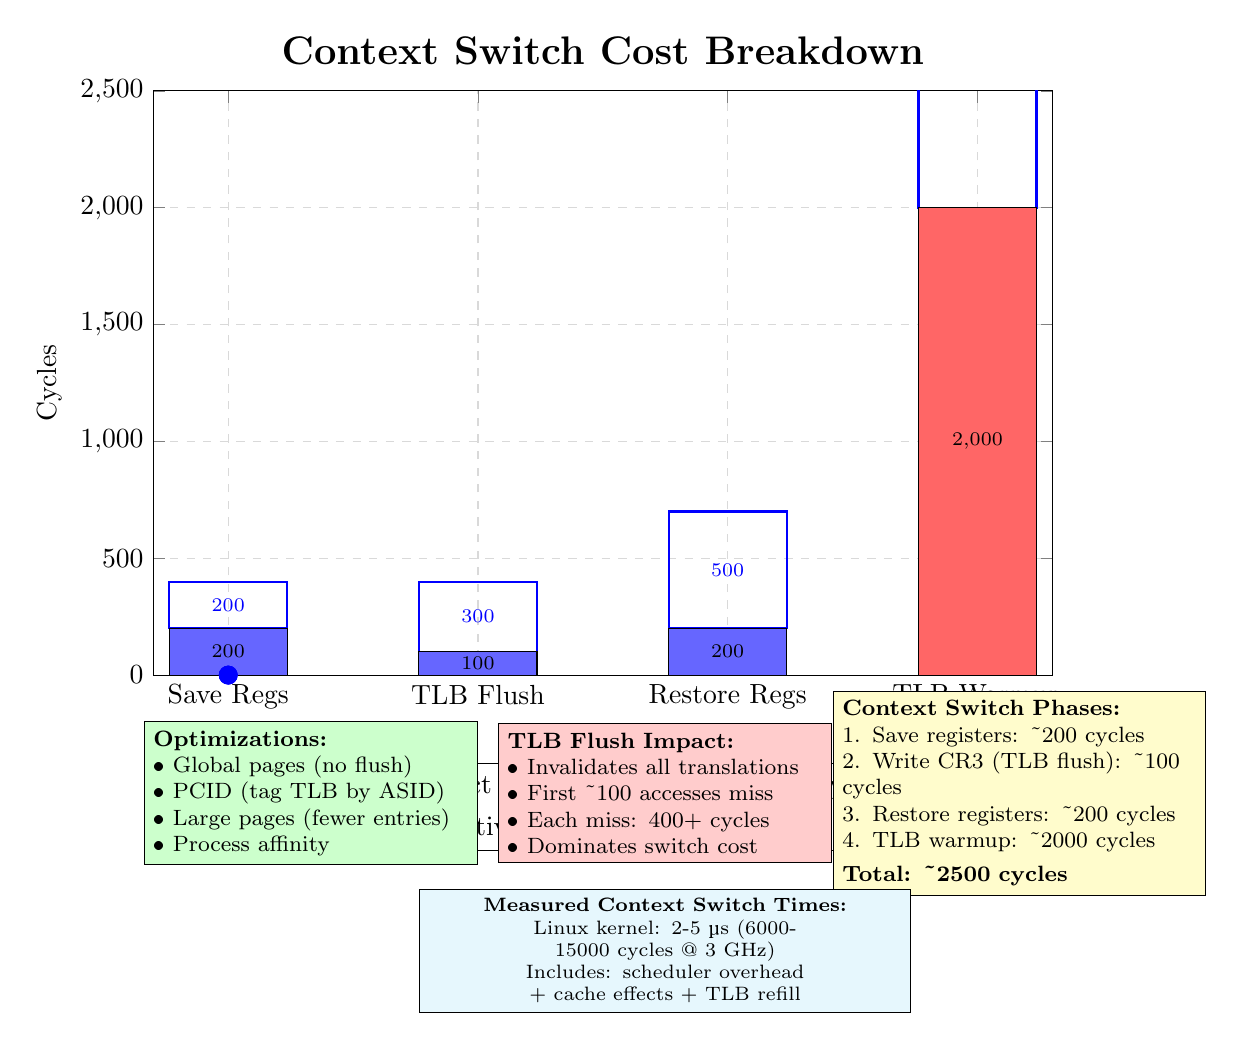
\begin{tikzpicture}
\begin{axis}[
    title={\Large\textbf{Context Switch Cost Breakdown}},
    xlabel={Component},
    ylabel={Cycles},
    ybar stacked,
    bar width=1.5cm,
    width=13cm,
    height=9cm,
    ymin=0,
    ymax=2500,
    xtick=data,
    symbolic x coords={Save Regs, TLB Flush, Restore Regs, TLB Warmup},
    legend style={at={(0.5,-0.15)},anchor=north,legend columns=2},
    grid=major,
    grid style={dashed,gray!30},
    nodes near coords,
    every node near coord/.append style={font=\scriptsize}
]

% Direct costs
\addplot[fill=blue!60] coordinates {
    (Save Regs, 200)
    (TLB Flush, 100)
    (Restore Regs, 200)
    (TLB Warmup, 0)
};
\addlegendentry{Direct Cost}

% TLB miss penalty
\addplot[fill=red!60] coordinates {
    (Save Regs, 0)
    (TLB Flush, 0)
    (Restore Regs, 0)
    (TLB Warmup, 2000)
};
\addlegendentry{TLB Miss Penalty}

% Total line
\addplot[thick,mark=*,mark size=3pt,blue] coordinates {
    (Save Regs, 200)
    (TLB Flush, 300)
    (Restore Regs, 500)
    (TLB Warmup, 2500)
};
\addlegendentry{Cumulative Total}

\end{axis}

% Cost breakdown annotation
\node[font=\footnotesize,fill=yellow!20,draw,text width=4.5cm,align=left] at (11,-1.5) {
    \textbf{Context Switch Phases:}\\
    1. Save registers: \textasciitilde200 cycles\\
    2. Write CR3 (TLB flush): \textasciitilde100 cycles\\
    3. Restore registers: \textasciitilde200 cycles\\
    4. TLB warmup: \textasciitilde2000 cycles\\
    \vspace{0.1cm}
    \textbf{Total: \textasciitilde2500 cycles}
};

% TLB impact
\node[font=\footnotesize,fill=red!20,draw,text width=4cm,align=left] at (6.5,-1.5) {
    \textbf{TLB Flush Impact:}\\
    • Invalidates all translations\\
    • First \textasciitilde100 accesses miss\\
    • Each miss: 400+ cycles\\
    • Dominates switch cost
};

% Mitigation strategies
\node[font=\footnotesize,fill=green!20,draw,text width=4cm,align=left] at (2,-1.5) {
    \textbf{Optimizations:}\\
    • Global pages (no flush)\\
    • PCID (tag TLB by ASID)\\
    • Large pages (fewer entries)\\
    • Process affinity
};

% Real-world data box
\node[font=\scriptsize,fill=cyan!10,draw,text width=6cm,align=center] at (6.5,-3.5) {
    \textbf{Measured Context Switch Times:}\\
    Linux kernel: 2-5 µs (6000-15000 cycles @ 3 GHz)\\
    Includes: scheduler overhead + cache effects + TLB refill
};

\end{tikzpicture}
\end{document}
